\documentclass[14pt]{article}
\usepackage[a4paper, margin=0.8in,top = 20mm,bottom = 20mm]{geometry}
\usepackage{enumerate}
\usepackage{subfigure}
\usepackage{amsmath}
\usepackage{algorithm}
\usepackage{algorithmic}
\usepackage{titlesec}
\usepackage{fancyhdr} % Required for custom headers
\usepackage{lastpage} % Required to determine the last page for the footer
\usepackage{subfig,graphicx} % Required to insert images
\usepackage{enumitem}
\usepackage{ctex}
% \usepackage{czt}
% \usepackage{hyperref}
\usepackage{zed-csp}

\numberwithin{figure}{subsection}
\pagestyle{fancy}
\lhead{网络空间安全一班} % Top left header
\chead{音乐管理系统} % Top center head
\rhead{谢远峰3019244283} % Top right heade
\renewcommand\headrulewidth{0.2pt} % Size of the header rule
\renewcommand\footrulewidth{0.4pt} % Size of the footer rul
\setlength{\headsep}{4mm}
\setlength{\footskip}{6mm}
% \titleformat{\section}[block]{\Large \bfseries}{\arabic{section}}{0.9em}{}[]
% \titleformat{\subsection}[block]{\large \bfseries}{\arabic{subsection}}{0.7em}{}[]
% \titleformat{\subsubsection}[block]{\large \bfseries}{ \arabic{subsubsection} }{0.4em}{}[]

\begin{document}

\begin{titlepage}
    \begin{center}
        \begin{figure}[H]
            \centering
            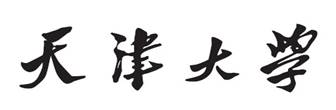
\includegraphics[width=6.048cm,height=1.98cm]{Content.png}
        \end{figure}
        \begin{figure}[H]
            \centering
            % \vspace{3cm}
            
\includegraphics[width=6.318cm,height=6.174cm]{Cover.png}
        \end{figure}
        \vspace*{2cm}
        \line(1,0){300}\\
        [0.05cm]
        \Huge{\bfseries 逻辑与形式化方法实验报告 }\\
        \line(1,0){300}\\
        \LARGE {音乐管理系统\\
        \today\\
        [0.5cm]

        \begin{tabular}{rl}
            学院 :        & 智能与计算学部 \\
            班级 :        & 网络安全一班   \\
            姓名        : & 谢远峰         \\
            学号       :  & 3019244283
        \end{tabular}
        }
    \end{center}

\end{titlepage}
\clearpage

\tableofcontents

\clearpage
\section{需求说明}
本次作业设计音乐管理系统,具体事务和用户需求如下
\begin{enumerate}
    \setlength{\itemsep}{0pt}
          \setlength{\parsep}{0pt}
          \setlength{\parskip}{0pt}
    \item 每个用户可以拥有多个歌单
    \item 用户可以添加或删除一个或多个歌单
    \item 用户可以在歌单内部添加或删除一个或多个歌曲
    \item 用户可以通过音乐的作者或者主题查询音乐的具体信息
    \item 用户可以查看当前播放音乐的具体信息
    \item 用户可以暂停音乐的播放
    \item 用户可以切换下一首音乐播放
\end{enumerate}

同时,系统还需满足如下要求:

\begin{itemize}
    \setlength{\itemsep}{0pt}
          \setlength{\parsep}{0pt}
          \setlength{\parskip}{0pt}
    \item 歌单内的歌曲要么未播放,要么正在播放
    \item 不存在某个歌曲既处于播放状态,又处于未播放状态
    \item 用户可以创建的歌单数量具有上限
    \item 用户单个歌单内可以包含的歌曲数量具有上限
    \item 用户在当前时刻只能播放一首音乐
\end{itemize}

\section{形式规格说明}
\subsection{类型}
\centerline{[PERSON,LIST,MUSIC,AUTHOR,TITLE,SUBJECT]}

PERSON是所有可能的人的集合。LIST是所有歌单的集合。MUSIC是歌单内所有音乐的集合。AUTHOR是
所有可能的作者的集合。TITLE是所有可能音乐名称的的集合。SUBJECT是所有可能的主题的集合。
\vspace*{0.5cm}

Repert::=$ \verb|'| Success \verb|'| | \verb|'| Unknown\_User \verb|'| |
    \verb|'| Too\_Many\_Playlist \verb|'| | \verb|'| Too\_Many\_Music \verb|'|
    | \verb|'| Music\_Not\_In \verb|'| |
    \verb|'| Music\_Is\_Playing \verb|'| | \verb|'| Music\_Is\_Playing \verb|'| |
    \verb|'| Playlist\_In\_Account \verb|'| | \verb|'| Playlist\_Not\_In \verb|'|
$

添加特定的类型REPORT,它是所有必要信息的集合,可由以上枚举类型来进行定义
\subsection{常量}
\centerline{$| Playlist\_Limit, Music\_Limit:\ \nat$}

Playlist\_Limit表示用户最多可以创建的歌单数量,Music\_Limit表示用户在单个歌单内可以最多
添加的歌曲数量
\subsection{状态模式}
\vspace{-1cm}
\begin{figure}[h]
    \setlength{\abovecaptionskip}{0.cm}
    \setlength{\belowcaptionskip}{0.cm}
    \begin{schema}{USER}
        user: \power PERSON\\
        manager: \power PERSON\\
        \where
        user \cap manager = \emptyset
    \end{schema}
    \caption{用户状态模式USER}
\end{figure}

模式USER定义了用户状态,其中user表示普通用户,manager表示管理员用户
,规定两种用户无交集

\clearpage
\vspace{-1cm}
\begin{figure}[ht]
    \setlength{\abovecaptionskip}{0.cm}
    \setlength{\belowcaptionskip}{0.cm}
    \begin{schema}{STORE}
        list\_title:TITLE\\
    \end{schema}
    \caption{模式STORE:定义歌单的基本信息}
\end{figure}

\vspace{-1.3cm}
\begin{figure}[ht]
    \setlength{\abovecaptionskip}{0.cm}
    \setlength{\belowcaptionskip}{0.cm}
    \begin{schema}{SONG}
        title:TITLE\\
        author:\finset\ AUTHOR\\
        subjects:\finset \ SUBJECT\\
    \end{schema}
    \caption{模式SONG:定义歌曲的基本信息}
\end{figure}

\vspace{-1.3cm}
\begin{figure}[H]
    \setlength{\abovecaptionskip}{0.cm}
    \setlength{\belowcaptionskip}{0.cm}
    \begin{schema}{DB}
        account: \power LIST\\
        playlist:\power MUSIC\\
        unplay:\power MUSIC\\
        playing: \power MUSIC \pfun PERSON\\
        last\_playing:\power MUSIC \pfun PERSON\\
        music\_info:MUSIC \pfun SONG\\
        list\_info:LIST \pfun STORE\\
        \where
        (\dom \ playing)\cup unplay\ = playlist\\
        (\dom \ playing)\cap unplay\ = \emptyset\\
        \forall p: PERSON @ \#~(playing \rres \{p\})\subseteq\ \{0,1\}\\
        playing \subseteq \ last\_playing\\
        \dom music\_info\ =\ playlist\\
        \dom list\_info\ =\ account\\
    \end{schema}
    \caption{数据库状态模式DB:描述歌单和播放信息的数据库状态}
\end{figure}

\vspace{-1.3cm}
\begin{figure}[H]
    \setlength{\abovecaptionskip}{0.cm}
    \setlength{\belowcaptionskip}{0.cm}
    \begin{schema}{LIB}
        USER\\
        DB\\
        \where
        \ran playing \subseteq user
    \end{schema}
    \caption{数据库状态模式DB:描述歌单和播放信息的数据库状态}
\end{figure}
\vspace{-1cm}
\begin{figure}[H]
    \setlength{\abovecaptionskip}{0.cm}
    \setlength{\belowcaptionskip}{0.cm}
    \begin{syntax}
        \Delta SONG \defs  SONG \wedge SONG'\\
        \Delta USER \defs  USER \wedge USER'\\
        \Delta DB \defs  DB \wedge DB'\\
        \Delta LIB \defs  LIB \wedge LIB'\\
        \Xi SONG \defs  \Delta SONG\ |\ title'=title \wedge author'=author \wedge subjects'=subjects\\
        \Xi USER \defs  \Delta SONG\ |\ user'=user \wedge manager'=manager \\
        \Xi DB \defs   \Delta DB\ |\ playlist'=playlist \wedge unplay'=unplay  \wedge \\
        \t3 \quad playing'=playing\ \wedge last\_playing'=last\_playing \wedge music\_info'=music\_info \wedge \ \\
        \t3 \quad account' = account \wedge list\_info' = list\_info\\
        \Xi LIB \defs  \Delta LIB\ |\ \theta USER'=\theta USER \wedge \theta DB'=\theta DB
    \end{syntax}
    \caption{状态模式定义:$\Delta SONG\ \Delta USER\ \Delta DB\ \Delta LIB\ \Xi SONG\ \Xi USER\ \Xi DB\ \Xi LIB$}
\end{figure}

\clearpage
\subsection{状态模式初始化}

系统初始化时,管理系统中使用用户,也无歌单和歌曲,但至少存在一个管理人员。由于需求
中并未要求增加管理人员和增加读者等“用户控制系统”的事务,故假定管理人员集合和用户
人员集合在初始化时已经设置好。可以假定管理员集合为\{happytraveller\_alone\},
普通用户集合为\{traveller1、traveller2\}
\vspace{-0.5cm}
\begin{figure}[H]
    \setlength{\abovecaptionskip}{0.cm}
    \setlength{\belowcaptionskip}{0.cm}
    \begin{schema}{InitUSER}
        USER'\\
        \where
        user' \neq \emptyset\\
        manager' \neq \emptyset\\
    \end{schema}
    \caption{用户集群初始化}
\end{figure}
\vspace{-1.5cm}
\begin{figure}[H]
    \setlength{\abovecaptionskip}{0.cm}
    \setlength{\belowcaptionskip}{0.cm}
    \begin{schema}{InitDB}
        DB'\\
        \where
        account'=\emptyset\\
        playlist'=\emptyset \\
        music\_info=\emptyset \\
        unplay'=\emptyset \\
        playing'=\emptyset \\
        last\_playing'=\emptyset\\
        list\_info'=\emptyset
    \end{schema}
    \caption{数据库初始化}
\end{figure}
\vspace{-1.5cm}
\begin{figure}[H]
    \setlength{\abovecaptionskip}{0.cm}
    \setlength{\belowcaptionskip}{0.cm}
    \begin{schema}{InitLIB}
        LIB'\\
        \where
        InitUSER \\
        InitDB \\
    \end{schema}
    \caption{组合模式初始化}
\end{figure}
\vspace{-0.3cm}
显然InitUSER初始化状态存在,故证明InitDB及InitLIB的初始化定理

% \vspace{0.3cm}
模式InitDB初始化定理可描述为$\vdash \exists DB' \bullet InitDB$

\begin{minipage}[t]{0.52\linewidth}
    展开该定理,可得下式(1)
    \begin{syntax}
        \vdash \exists playlist',unplay':\power MUSIC;\\
        \t1  account': LIST,list\_info: LIST\pfun STORE;\\
        \t1  playing',last\_playing: MUSIC \pfun PERSON;\\
        \t1  music\_info: MUSIC \pfun SONG\\
        \t1 \ (\dom \ playing)\cup unplay\ = playlist\\
        \t1 \ (\dom \ playing)\cap unplay\ = \emptyset\\
        \t1 \ \forall p: PERSON @ \#~(playing \rres \{p\})\subseteq\ \{0,1\}\\
        \t1 \ playing \subseteq \ last\_playing\\
        \t1 \ \dom music\_info\ =\ playlist @\\
        \t1 \ playlist'=\emptyset \wedge music\_info=\emptyset \wedge unplay'=\emptyset \ \wedge\\
        \t1 \ playing'=\emptyset \wedge last\_playing'=\emptyset
    \end{syntax}
\end{minipage}
\hfill
\begin{minipage}[t]{0.45\linewidth}
    消除“|”,并应用点规则,可得下式(2):
    \begin{argue}
        \vdash \emptyset \in \power MUSIC \wedge \\
        \t1 \emptyset \in \power LIST \wedge \emptyset \in \power MUSIC \wedge\\
        \t1 \emptyset \in \power LIST \pfun STORE \\
        \t1 \emptyset \in  \nat \pfun MUSIC \\
        \t1 \emptyset \in \power MUSIC \pfun PERSON\ \wedge\\
        \t1  \emptyset \in \power MUSIC \pfun PERSON \wedge \\
        \t1 \emptyset \in \power MUSIC \pfun SONG\\
        \t1 \emptyset \mapsto \emptyset\\
        \t1 (\dom \emptyset)\cup \emptyset = \emptyset \wedge (\dom \emptyset)\cap \emptyset = \emptyset\\
        \t1 \forall p: PERSON @ \#~(\emptyset \rres \{p\})\subseteq\ \{0,1\}\\
        \t1 \emptyset \subseteq \emptyset \wedge (\dom \emptyset) = \emptyset \wedge\dom \emptyset = \emptyset\\
    \end{argue}
\end{minipage}

\clearpage
\begin{minipage}[t]{0.5\linewidth}
    \begin{flushleft}
        子目标:
        \vspace{-0.5cm}
        \begin{syntax}
            (01) \vDash \emptyset \in \power MUSIC \\
            (02) \vDash \emptyset \in \power MUSIC  \\
            (03) \vDash \emptyset \in \power MUSIC \pfun PERSON  \\
            (04) \vDash \emptyset \in \power MUSIC \pfun PERSON \\
            (05) \vDash \emptyset \in \power MUSIC \pfun SONG \\
            (06) \vDash (\dom \emptyset)\cup \emptyset = \emptyset \\
            (07) \vDash (\dom \emptyset)\cap \emptyset = \emptyset \\
            (08) \vDash \forall p: PERSON @ \#~(\emptyset \rres \{p\})\subseteq\ \{0,1\} \\
            (09) \vDash \emptyset \subseteq \emptyset \\
            (10) \vDash \dom \emptyset = \emptyset \\
        \end{syntax}
    \end{flushleft}
\end{minipage}
\hfill
\begin{minipage}[t]{0.45\linewidth}
    \quad 子目标(1)(2)可通过定理12证明,子目标(3)(4)(5)利用定理14证明。
    (6)(7)利用定律16将$\dom \emptyset$重写为$\emptyset$,利用
    应用L19和L25可得到证明。(9)利用定律4证明,(10)由定律6证明,
    进行(8)的证明。\par
    \quad 使用定律L27,重写为$\forall P: PERSON \bullet \#~{\emptyset}\leq \{0,1\}$
    根据定理L28,$\# \emptyset = 0$,有$\forall P:PERSON \bullet 0 \leq \{0,1\}$\par
    \quad 由数学定理可知:$\forall P: PERSON \bullet true$得证。\par
    \quad InitDB初始化定理证毕。\par
\end{minipage}

模式InitLIB初始化定理可描述为$\vdash \exists LIB' \bullet InitLIB$

由于InitUSER和InitDB相互独立且成立,结合点规则,
可知InitLIB初始化状态存在
\subsection{操作模式}
用户需求事务可分为两种情况:管理人员事务与普通用户事务

\subsubsection{管理人员事务}
管理人员事务包括音乐管理事务,查询事务

所用管理人员事务包含以下特点:在不影响用户系统的前提下,需要管理
人员的名称,引入模式mana\_\\ger\_trans,LIB状态模式不受到改变。
\vspace{-0.5cm}
\begin{figure}[H]
    \setlength{\abovecaptionskip}{0.cm}
    \setlength{\belowcaptionskip}{0.cm}
    \begin{schema}{manager\_trans}
        \Delta LIB\\
        id?: PERSON
        \where
        id? \in manager\\
        \theta USER' = \theta USER
    \end{schema}
    \caption{管理人员事务模式manager\_trans}
\end{figure}
\vspace*{-0.5cm}
(1)歌单管理事务

歌单管理事务包括歌单的添加,删除,与歌单名称相关,引入管理事务account\_manage。
\vspace{-0.5cm}
\begin{figure}[H]
    \setlength{\abovecaptionskip}{0.cm}
    \setlength{\belowcaptionskip}{0.cm}
    \begin{schema}{account\_manage}
        account\_manage\\
        account?: LIST
        \where
        playlist' = playing
    \end{schema}
    \caption{管理人员歌单管理事务模式account\_manage}
\end{figure}
\vspace*{-0.5cm}
歌单删除事务需给确保用户包含歌单playlist?,需要修改account'和list\_info的记录

\vspace{-0.5cm}
\begin{figure}[H]
    \setlength{\abovecaptionskip}{0.cm}
    \setlength{\belowcaptionskip}{0.cm}
    \begin{schema}{playlist\_remove}
        account\_manage\\
        \where
        playlist? \in account\\
        account' = account \setminus (playlist?)\\
        list\_info' = \{playlist\} \ndres list\_info
    \end{schema}
    \caption{管理人员歌单管理删除事务模式playlist\_remove}
\end{figure}

\clearpage
歌单添加事务需给定歌单的名称playlist?,并提供歌单的名称。

\vspace{-0.5cm}
\begin{figure}[H]
    \setlength{\abovecaptionskip}{0.cm}
    \setlength{\belowcaptionskip}{0.cm}
    \begin{schema}{playlist\_add}
        account\_manage\\
        playlist\_tilte?: TITLE
        \where
        playlist? \not\in account\\
        account' = account \cup (playlist?)\\
        list\_info' = list\_info \oplus \{playlist \mapsto B\}\\
        \t1 where\ B:STORE\ |\ B.playlist\_tilte=playlist\_tilte?\\
    \end{schema}
    \caption{管理人员歌单管理添加事务模式playlist\_add}
\end{figure}

\vspace{-0.5cm}
(2)音乐管理事务

音乐管理事务包括歌单内音乐的添加,删除,且不影响用户歌曲播放,引入音乐管理事务music\_manage。
\vspace{-0.5cm}
\begin{figure}[H]
    \setlength{\abovecaptionskip}{0.cm}
    \setlength{\belowcaptionskip}{0.cm}
    \begin{schema}{music\_manage}
        music\_manage\\
        music?: MUSIC\\
        \where
        playing' = playing\\
    \end{schema}
    \caption{管理人员歌曲管理事务模式music\_manage}
\end{figure}

\vspace*{-0.5cm}
歌曲删除事务需给确保用户包含歌曲music?,需要修改unplay'和music\_info的记录
\vspace{-0.7cm}
\begin{figure}[H]
    \setlength{\abovecaptionskip}{0.cm}
    \setlength{\belowcaptionskip}{0.cm}
    \begin{schema}{music\_remove}
        music\_manage\\
        \where
        music? \in playlist\\
        playlist' = playlist \setminus (music?)\\
        unplay' = unplay \setminus (music?)\\
        last\_playing' = last\_playing\\
        music\_info' = \{music?\} \ndres music\_info
    \end{schema}
    \caption{管理人员歌曲管理删除事务模式music\_remove}
\end{figure}

\vspace{-0.5cm}
歌曲添加事务需给定歌曲music?,并提供歌曲的名称,歌曲的作者,歌曲的主题
\vspace{-0.7cm}
\begin{figure}[H]
    \setlength{\abovecaptionskip}{0.cm}
    \setlength{\belowcaptionskip}{0.cm}
    \begin{schema}{music\_add}
        music\_manage\\
        tilte?: TITLE\\
        author?: \finset AUTHOR\\
        subjects?: \finset SUBJECT\\
        \where
        music? \not\in playlist\\
        playlist' = playlist \cup (music?)\\
        unplay' = unplay \cup (music?)\\
        last\_playing' = last\_playing\\
        music\_info' = music\_info \oplus \{music \mapsto m\}\\
        \t1 where\ m:SONG\ |\ SONG.tilte=tilte?\\
        \t5 \quad SONG.author = author?\\
        \t5 \quad SONG.subjects = subjects?
    \end{schema}
    \caption{管理人员歌曲管理添加事务模式music\_add}
\end{figure}

\clearpage
(2)查询事务

查询事务不影响音乐播放的状态

操作模式Manage\_list可通过用户标志operator?查找用户对于账户的操作,
查阅结果list!是音乐信息的集合
\vspace{-0.7cm}
\begin{figure}[H]
    \setlength{\abovecaptionskip}{0.cm}
    \setlength{\belowcaptionskip}{0.cm}
    \begin{schema}{Manage\_list}
        music\_manage\\
        operator?:PERSON\\
        list!:\finset (MUSIC\ \times\ SONG)
        \where
        operator? \in manager \cup user\\
        list! = \{c: MUSIC\ | playing(c)= operator? @ (c,music\_info(c))\}
    \end{schema}
    \caption{管理人员歌曲查询事务模式Manage\_list}
\end{figure}

\subsubsection{普通用户事务}
普通用户事务包括音乐查询事务,音乐播放事务

所用普通用户事务包含以下特点:可以查询音乐和播放音乐,引入模式User\_trans
,LIB状态模式不受到改变。

\begin{figure}[H]
    \setlength{\abovecaptionskip}{0.cm}
    \setlength{\belowcaptionskip}{0.cm}
    \begin{schema}{User\_trans}
        \Delta LIB\\
        id?: PERSON
        \where
        id? \in user \cup manager\\
        \theta LIB' = \theta LIB
    \end{schema}
    \caption{普通用户人员事务模式User\_trans}
\end{figure}

查询歌曲作者信息以满足给定描述或者主题信息满足给定的音乐信息集合
引入给定描述与歌手信息对应关系和给定描述与主题信息的相关信息

[DESC]
\vspace*{-0.2cm}
\begin{axdef}
    A\_match: DESC\leftrightarrow AUTHOR\\
    S\_match: DESC\leftrightarrow SUBJECT
\end{axdef}

(1)歌曲查询事务

用户可以通过歌手信息描述查询歌曲,Author\_enquriy根据用户输入的歌手信息描述d?,
给出关于歌手的所有歌曲信息
\vspace{-0.5cm}
\begin{figure}[H]
    \setlength{\abovecaptionskip}{0.cm}
    \setlength{\belowcaptionskip}{0.cm}
    \begin{schema}{Author\_enquiry}
        User\_trans\\
        d?:DESC\\
        list!: \power MUSIC
        \where
        list!=\{m:MUSIC|m \in \ran music\_info \wedge (m.author \cap A\_match(d?)\neq \emptyset)\}
    \end{schema}
    \caption{普通用户查询操作模式Author\_enquiry}
\end{figure}

\clearpage
用户可以通过主题信息描述查询歌曲,Subject\_enquriy根据用户输入的主题信息描述d?,
给出关于主题的所有歌曲信息

\vspace{-0.5cm}
\begin{figure}[H]
    \setlength{\abovecaptionskip}{0.cm}
    \setlength{\belowcaptionskip}{0.cm}
    \begin{schema}{Subject\_enquriy}
        User\_trans\\
        d?:DESC\\
        list!: \power MUSIC
        \where
        list!=\{m:MUSIC|m \in \ran music\_info \wedge (m.subjects \cap S\_match(d?)\neq \emptyset)\}
    \end{schema}
    \caption{普通用户查询操作模式Subject\_enquriy}
\end{figure}

用户可以播放已管理的歌曲,Playing\_music进行歌曲播放
\vspace{-0.5cm}
\begin{figure}[H]
    \setlength{\abovecaptionskip}{0.cm}
    \setlength{\belowcaptionskip}{0.cm}
    \begin{schema}{Playing\_music}
        User\_trans\\
        out!: \power MUSIC
        \where
        out!=\{m:MUSIC|m \in \dom playing \}
    \end{schema}
    \caption{普通用户音乐播放模式Playing\_music}
\end{figure}

\subsection{操作模式前置条件}
\vspace{-0.5cm}
\begin{figure}[H]
    \setlength{\abovecaptionskip}{0.cm}
    \setlength{\belowcaptionskip}{0.cm}
    \begin{schema}{Pre\_account\_add}
        LIB?;\\
        id?:PERSON\\
        playlist?:LIST\\
        playlist\_title?:TITLE
        \where
        id? \in manager\\
        % playlist? \not \in account
        playlist\_title? \not \in \ran list_info
    \end{schema}
    \caption{前置条件模式Pre\_account\_add}
\end{figure}
\vspace{-0.5cm}
\begin{figure}[H]
    \setlength{\abovecaptionskip}{0.cm}
    \setlength{\belowcaptionskip}{0.cm}
    \begin{schema}{Pre\_account\_remove}
        LIB;\\
        id?:PERSON\\
        playlist?:LIST\\
        playlist\_title?:TITLE
        \where
        id? \in manager\\
        playlist\_title? \in \ran list_info
    \end{schema}
    \caption{前置条件模式Pre\_account\_remove}
\end{figure}
\vspace{-0.5cm}
\begin{figure}[H]
    \setlength{\abovecaptionskip}{0.cm}
    \setlength{\belowcaptionskip}{0.cm}
    \begin{schema}{Pre\_music\_add}
        LIB;\\
        id?:PERSON\\
        music:MUSIC\\
        title?:TITLE\\
        author?:\ndres AUTHOR\\
        subjects?:\ndres SUBJECT\\
        \where
        id? \in manager\\
        music? \not \in unplay\\
        music? \not \in playlist
    \end{schema}
    \caption{前置条件模式Pre\_music\_add}
\end{figure}
\vspace{-1cm}
\begin{figure}[H]
    \setlength{\abovecaptionskip}{0.cm}
    \setlength{\belowcaptionskip}{0.cm}
    \begin{schema}{Pre\_music\_remove}
        LIB;\\
        id?:PERSON\\
        music:MUSIC\\
        \where
        id? \in manager\\
        music?  \in unplay
        music?  \in playlist
    \end{schema}
    \caption{前置条件模式Pre\_music\_remove}
\end{figure}
\vspace{-1cm}
\begin{figure}[H]
    \setlength{\abovecaptionskip}{0.cm}
    \setlength{\belowcaptionskip}{0.cm}
    \begin{schema}{Pre\_Author\_enquiry}
        LIB;\\
        id?:PERSON\\
        d?:DESC\\
        \where
        id? \in manager \cup user
    \end{schema}
    \caption{前置条件模式Pre\_Author\_enquiry}
\end{figure}
\vspace{-1cm}
\begin{figure}[H]
    \setlength{\abovecaptionskip}{0.cm}
    \setlength{\belowcaptionskip}{0.cm}
    \begin{schema}{Pre\_Subject\_enquiry}
        LIB;\\
        id?:PERSON\\
        d?:DESC\\
        \where
        id? \in manager \cup user
    \end{schema}
    \caption{前置条件模式Pre\_Subject\_enquiry}
\end{figure}
\vspace{-1cm}
\begin{figure}[H]
    \setlength{\abovecaptionskip}{0.cm}
    \setlength{\belowcaptionskip}{0.cm}
    \begin{schema}{Pre\_Playing}
        LIB;\\
        id?:PERSON\\
        \where
        id? \in \ran manager \cup user\\
        \dom playing \neq \emptyset
    \end{schema}
    \caption{前置条件模式Pre\_Playing}
\end{figure}
\clearpage
选取前置条件模式Pre\_music\_add进行证明证明
\vspace{-0.7cm}
\begin{figure}[H]
    \setlength{\abovecaptionskip}{0.cm}
    \setlength{\belowcaptionskip}{0.cm}
    \begin{schema}{music\_add}
        music\_manage\\
        id?: \power PERSON\\
        tilte?: TITLE\\
        author?: \finset AUTHOR\\
        subjects?: \finset SUBJECT\\
        \where
        \exists music\_manage;\ \bullet \\
        (music? \not\in playlist\\
        music? \not\in unplay\\
        playlist' = playlist \cup (music?)\\
        unplay' = unplay \cup (music?)\\
        last\_playing' = last\_playing\\
        music\_info' = music\_info \oplus \{music \mapsto m\}\\
        \t1 where\ m:SONG\ |\ SONG.tilte=tilte?\\
        \t5 \quad SONG.author = author?\\
        \t5 \quad SONG.subjects = subjects?)
    \end{schema}
\end{figure}
\vspace{-0.7CM}
考虑该模式的谓词部分,因为$music? \not\in playlist\ \&\&\ unplay$ 由点规则得到
$playlist' = unplay/playlist \cup (music?)$,且$last\_playing=last\_playing$
故可对1,2,3式进行消去
\vspace{-0.7cm}
\begin{figure}[H]
    \setlength{\abovecaptionskip}{0.cm}
    \setlength{\belowcaptionskip}{0.cm}
    \begin{schema}{music\_add}
        music\_manage\\
        id?: \power PERSON\\
        tilte?: TITLE\\
        author?: \finset AUTHOR\\
        subjects?: \finset SUBJECT\\
        \where
        \exists music\_manage; \bullet \\
        (music\_info' = music\_info \oplus \{music \mapsto m\}\\
        \t1 where\ m:SONG\ |\ SONG.tilte=tilte?\\
        \t5 \quad SONG.author = author?\\
        \t5 \quad SONG.subjects = subjects?)
    \end{schema}
\end{figure}

\vspace{-0.7CM}
因为$m.title:TITLE,m.author:AUTHOR,m.subjects:SUBJECT,m:MUSIC$
并且$music\oplus \not \in music\_info$,\\所以$music\_info'\equiv music\_info \oplus \{music\mapsto m\}\}$,
进行消去。同时,添加的author,subjects应当属于尚未添加的属性,故在定义域上添加$\ndres$,证明完毕

\vspace{-0.7cm}
\begin{figure}[H]
    \setlength{\abovecaptionskip}{0.cm}
    \setlength{\belowcaptionskip}{0.cm}
    \begin{schema}{Pre\_music\_add}
        LIB;\\
        id?:PERSON\\
        music:MUSIC\\
        title?:TITLE\\
        author?:\ndres AUTHOR\\
        subjects?:\ndres SUBJECT\\
        \where
        id? \in manager\\
        music? \not \in playlist\\
        music? \not \in unplay
    \end{schema}
\end{figure}
\subsection{操作的完整性描述和出错处理}
\begin{minipage}[t]{0.5\linewidth}
    \begin{flushleft}
        模式Error
        \vspace*{-0.5cm}
        \begin{schema}{Error}
            \Delta LIB;\\
            r!:REPORT
            \where
            \theta LIB =\theta LIB'\\
        \end{schema}
        \vspace*{-0.5cm}
        模式Success
        \vspace*{-0.1cm}
        \begin{schema}{Success}
            rep!:REPORT
            \where
            rep!:'Success'
        \end{schema}
        \vspace*{-0.5cm}
        模式Unknown\_User
        \vspace*{-0.1cm}
        \begin{schema}{Unknown\_User}
            Error\\
            id?:PERSON
            \where
            id? \not \in manager \cup user\\
            r!:= 'Unknown\_User'
        \end{schema}
        \vspace*{-0.5cm}
        模式Too\_Many\_Playlist
        \vspace*{-0.1cm}
        \begin{schema}{Too\_Many\_Playlist}[\hspace{-0.7cm}]
            Error\\
            id?:PERSON
            \where
            \#~(account) \geq Playlist\_Limit\\
            r!:='Too\_Many\_Playlist'
        \end{schema}
        \vspace*{-0.5cm}
        模式Too\_Many\_Music
        \vspace*{-0.1cm}
        \begin{schema}{Too\_Many\_Music}
            Error\\
            id?:PERSON
            \where
            \#~(playlist) \geq Music\_Limit\\
            r!:='Too\_Many\_Music
        \end{schema}
        添加M\_Error,描述音乐不在当前歌单内的状态
        \begin{syntax}
            M\_Error\defs  [Error \comp \ music?:MUSIC]
        \end{syntax}
        \vspace{-1.5cm}
        \begin{figure}[H]
            \setlength{\abovecaptionskip}{0.cm}
            \setlength{\belowcaptionskip}{0.cm}
            \begin{schema}{Music\_Not\_In}
                M\_Error
                \where
                (music? \not\in playlist \wedge r!)='Music\_Not\_In')\\
                \vee \ (music? \in playlist \setminus unplay \wedge\\
                r!\ =\ 'Music\_Is\_Playing')
            \end{schema}
            \caption{模式Music\_Not\_In}
        \end{figure}
    \end{flushleft}
\end{minipage}
\hfill
\begin{minipage}[t]{0.5\linewidth}
    \begin{flushleft}
        添加A\_Error,描述不存在歌单内的状态
        \begin{syntax}
            A\_Error\defs  [Error \comp \ playlist?:MUSIC]
        \end{syntax}
        \vspace{-1.5cm}
        \begin{figure}[H]
            \setlength{\abovecaptionskip}{0.cm}
            \setlength{\belowcaptionskip}{0.cm}
            \begin{schema}{Playlist\_Not\_In}
                A\_Error
                \where
                (playlist? \not\in account \wedge r!)='Playlist\_Not\_In')
            \end{schema}
            \caption{模式Playlist\_Not\_In}
        \end{figure}

        定义音乐播放的完整操作描述为:
        \begin{syntax}
            \hspace{-0.7cm}
            T\_Playing \defs  (Music\_Playing \wedge Success)\\
            \t1 \vee Unknown\_User\\
            \t1 \vee Too\_Mang\_Music\\
            \t1 \vee Music\_Not\_In\\
        \end{syntax}

        定义歌单在账户中的完整操作描述为:
        \begin{syntax}
            \hspace{-0.7cm}
            Playlist\_In\_Account \defs  [A\_Error\ |playlist? \in account \\
                \t2 \wedge r! = 'Playlist\_In\_Account']
        \end{syntax}

        定义音乐在播放列表中完整描述为:
        \begin{syntax}
            \hspace{-0.7cm}
            Music\_In\_Playlist \defs  [M\_Error\ |music? \in playlist \\
                \t2 \wedge r! = 'Music\_In\_Playlist']
        \end{syntax}

        添加歌单操作模式
        \begin{syntax}
            \hspace{-0.7cm}
            Playlist\_Add \defs  (playlist\_add \wedge Success)\\
            \t1 \vee Unknown\_manager\\
            \t1 \vee Playlist\_In\_Account
        \end{syntax}

        删除歌单操作模式
        \begin{syntax}
            \hspace{-0.7cm}
            Playlist\_Remove \defs  (playlist\_remove \wedge Success)\\
            \t1 \vee Unknown\_manager\\
            \t1 \vee Playlist\_Not\_In
        \end{syntax}


        添加音乐操作模式
        \begin{syntax}
            \hspace{-0.7cm}
            Music\_Add \defs  (music\_add \wedge Success)\\
            \t1 \vee Unknown\_manager\\
            \t1 \vee Playlist\_In\_account
        \end{syntax}

        删除音乐操作模式
        \begin{syntax}
            \hspace{-0.7cm}
            Music\_Remove \defs  (music\_remove \wedge Success)\\
            \t1 \vee Unknown\_manager\\
            \t1 \vee Music\_Not\_In
        \end{syntax}
    \end{flushleft}
\end{minipage}

\clearpage
\section{规格说明的性质和证明}
% \vspace*{-1cm}
管理员添加一个有效的歌曲并立即删除,不会导致歌单信息的状态改变

可表示为如下定理:$music\_add \comp \ music\_remove \| id?\ music?\ title?\ author?\ subjects?
    \vDash \Xi DB$

记录新模式$music\_add \comp \ music\_remove$为AddAndRemove

\begin{minipage}[t]{0.5\linewidth}
    \begin{schema}{music\_remove}
        music\_manage\\
        \where
        music? \in playlist\\
        playlist' = playlist \setminus (music?)\\
        unplay' = unplay \setminus (music?)\\
        last\_playing' = last\_playing\\
        music\_info' = \{music?\} \ndres music\_info
    \end{schema}
\end{minipage}
\hfill
\begin{minipage}[t]{0.5\linewidth}
    \begin{schema}{music\_add}
        music\_manage\\
        tilte?: TITLE\\
        author?: \finset AUTHOR\\
        subjects?: \finset SUBJECT\\
        \where
        music? \not\in playlist\\
        playlist' = playlist \cup (music?)\\
        unplay' = unplay \cup (music?)\\
        last\_playing' = last\_playing\\
        music\_info' = music\_info \oplus \{music \mapsto m\}\\
        \t1 where\ m:SONG\ |\ SONG.tilte=tilte?\\
        \t3 \quad SONG.author = author?\\
        \t3 \quad SONG.subjects = subjects?
    \end{schema}

\end{minipage}

\begin{schema}{AddAndRemove}
    \Delta DB\\
    id?: PERSON\\
    music?: MUSIC\\
    title?: TITLE\\
    author?: AUTHOR\\
    subjects?: SUBJECT\\
    \where
    \exists DB\plus @(\\
    id? \in manager\\
    music? \not \in playlist\\
    playlist\plus = playlist \cup (music?)\\
    last\_playing\plus = last\_playing
    music\_info\oplus = music\_info \oplus \{music \mapsto m\}\\
    \t1 where\ m:SONG\ |\ SONG.tilte=tilte?\\
    \t5 \quad SONG.author = author?\\
    \t5 \quad SONG.subjects = subjects?\\
    music? \in playlist\plus \\
    playlist' = playlist\plus \setminus (music?)\\
    unplay' = unplay\plus \setminus (music?)\\
    last\_playing' = last\_playing\plus \\
    music\_info' = \{music?\} \ndres music\_info\plus\\
    )
\end{schema}
展开该定理
\begin{schema}{AddAndRemove}
    \Delta DB\\
    id?: PERSON\\
    music?: MUSIC\\
    title?: TITLE\\
    author?: AUTHOR\\
    subjects?: SUBJECT
    \where
    \exists DB\plus ;
    account: \power LIST\\
    playlist:\power MUSIC\\
    unplay:\power MUSIC\\
    playing: MUSIC \pfun PERSON\\
    last\_playing:\power MUSIC \pfun PERSON\\
    music\_info:\power MUSIC \pfun SONG\\
    list\_info:\power LIST \pfun STORE\ @(\\
    id? \in manager\\
    music? \not \in playlist\\
    playlist\plus = playlist \cup (music?)\\
    last\_playing\plus = last\_playing\\
    music\_info\oplus = music\_info \oplus \{music \mapsto m\}\\
    \t1 where\ m:SONG\ |\ SONG.tilte=tilte?\\
    \t5 \quad SONG.author = author?\\
    \t5 \quad SONG.subjects = subjects?\\
    music? \in playlist\plus \\
    playlist' = playlist\plus \setminus (music?)\\
    unplay' = unplay\plus \setminus (music?)\\
    last\_playing' = last\_playing\plus \\
    music\_info' = \{music?\} \ndres music\_info\plus\\
    )
\end{schema}

因为last\_playing'=last\_playing ,playing'=playing
list\_info'=list\_info 故可消去

现在证明,下式不会导致状态的改变

\begin{syntax}
    music\_info' = \{music?\} \ndres (music\_info \oplus \{music \mapsto m\\
    \t1 where\ m:SONG\ |\ SONG.tilte=tilte?\\
    \t5 \quad SONG.author = author?\\
    \t5 \quad SONG.subjects = subjects?)\}\\
    playlist'= playlist \cup (music?) \setminus (music?)\\
    unplay' = unplay \cup (music?) \setminus (music?)\\
\end{syntax}

因为取并集后再进行删除,可知$playlist'=playlist,unplay'=unplay$

得证

\end{document}
